\documentclass[a4paper, 12pt, twoside, openany]{article}

% Pakiety
\usepackage[utf8]{inputenc}
\usepackage[T1]{fontenc}
\usepackage[polish]{babel}
\usepackage[hidelinks]{hyperref} % Hiperłącza bez ramek
%\usepackage{hyperref} % Hiperłącza
\usepackage{amsmath, amssymb} % Pakiety matematyczne
\usepackage{mathtools}
\usepackage{graphicx} % Obsługa grafiki
\graphicspath{{../img/}}
\usepackage{enumitem}
%\usepackage{fontspec}
\usepackage{float}
\usepackage[font=footnotesize,labelfont=bf]{caption}
\usepackage{setspace}
\usepackage{geometry} % Ustawienia marginesów
\geometry{
	inner=20mm, % margines wewnętrzny
	outer=20mm, % margines zewnętrzny
	top=25mm,   % margines górny
	bottom=25mm % margines dolny
}
\usepackage{cellspace} %
\setlength\cellspacetoplimit{100pt}
\setlength\cellspacebottomlimit{100pt}
\usepackage{xcolor}   % Pakiet do kolorów
\usepackage{listingsutf8} % Pakiet do listingu kodu
\lstdefinestyle{mystyle}{
	inputencoding=utf8,           % Kodowanie UTF-8
	extendedchars=true,           % Obsługa znaków spoza ASCII
	basicstyle=\ttfamily\footnotesize,   % Styl podstawowy
	language=Matlab,              % Język kodu
	keywordstyle=\bfseries\color{blue}, % Styl słów kluczowych
	commentstyle=\itshape\color{green!50!black}, % Styl komentarzy
	stringstyle=\color{red},      % Styl tekstu w cudzysłowach
	numbers=left,                 % Numeracja linii po lewej stronie
	numberstyle=\color{gray},     % Styl numerów linii
	frame=single,                 % Ramka wokół kodu
	breaklines=false,             % Zawijanie linii
	backgroundcolor=\color{gray!10}, % Kolor tła
	tabsize=2,                    % Wielkość tabulacji
	showstringspaces=false,        % Ukrywanie spacji w ciągach tekstowych
	literate={ą}{{\k{a}}}1
	{Ą}{{\k{A}}}1
	{ć}{{\'{c}}}1
	{Ć}{{\'{C}}}1
	{ę}{{\k{e}}}1
	{Ę}{{\k{E}}}1
	{ł}{\l}1
	{Ł}{\L}1
	{ń}{{\'{n}}}1
	{Ń}{{\'{N}}}1
	{ó}{{\'{o}}}1
	{Ó}{{\'{O}}}1
	{ś}{{\'{s}}}1
	{Ś}{{\'{S}}}1
	{ź}{{\'{z}}}1
	{Ź}{{\'{Z}}}1
	{ż}{{\.{z}}}1
	{Ż}{{\.{Z}}}1
}
\lstset{style=mystyle}

\renewcommand{\figurename}{Rys}

\newcommand{\y}{\mathbf{y}}
\newcommand{\I}{\mathbf{I}}
\newcommand{\A}{\mathbf{A}}
\newcommand{\f}{\mathbf{f}}
\renewcommand{\b}{\mathbf{b}}


\newcommand{\tytul}{Estymacja parametrów modelu}
\newcommand{\autor}{Wiktor Murawski}
\newcommand{\uczelnia}{Politechnika Warszawska}
\newcommand{\wydzial}{Wydział Matematyki i Nauk Informacyjnych}
\newcommand{\prowadzacy}{dr inż. Jakub Wagner}
\newcommand{\przedmiot}{Modelowanie matematyczne}
\newcommand{\miejsce}{Warszawa}
\date{\today}

% Dokument
\begin{document}
	
	% STRONA TYTUŁOWA
	\begin{titlepage}
		\centering
		\vspace*{1cm}
		\LARGE\textbf \tytul \\
		\vspace{1.5cm}
		\large
		%\normalsize
		Autor: \autor \\
		\vspace{1cm}
		Przedmiot: \przedmiot \\
		Prowadzący: \prowadzacy \\
		\vspace{2cm}
		\uczelnia \\
		\wydzial \\
		\vspace{2cm}
		Oświadczam, że niniejsza praca, stanowiąca podstawę do uznania osiągnięcia efektów
		uczenia się z przedmiotu Modelowanie matematyczne, została wykonana przeze mnie samodzielnie.\\
		\vspace{2cm}
		\miejsce \\
		\today \\
	\end{titlepage}
	
	% SPIS TREŚCI
	\tableofcontents
	\newpage
	
	% Lista symboli i akronimów
	\section{Lista Symboli i Akronimów}
	%\addcontentsline{toc}{section}{Lista Symboli i Akronimów}
	\begin{spacing}{1.5}
		\begin{tabbing}
			\hspace{5cm} \= \hspace{10cm} \= \kill
			\text{URRZ} \> układ równań różniczkowych zwyczajnych \\
			$t$ \> czas \\
			$x_k(t)$ i $y_k(t)$ \> współrzędne położenia $k$-tego obiektu w chwili $t$\\
			$m$ \> masa obiektu \\
			$G$ \> stała grawitacyjna \\
			$r_{jk}(t)$ \> odległość pomiędzy obiektami $j$ i $k$ dla $j,k = 1,2,3$ w chwili $t$.
		\end{tabbing}
	\end{spacing}
	\newpage
	
	% Wprowadzenie
	\section{Wprowadzenie}
	
	Dane zawarte w pliku \texttt{data\_30.csv} reprezentują wyniki pomiaru położenia trzech obiektów o
	identycznych masach $m$, przyciągających się grawitacyjnie. Trajektorie ruchu tych obiektów opisane
	są następującym układem nieliniowych równań różniczkowych zwyczajnych drugiego rzędu:\\
	\begin{equation}	
		\label{eq1}
		\hspace{-5cm}
		\left\{
		\begin{alignedat}{4}
			\dfrac{d^2x_1(t)}{dt^2} & = Gm \Big( & \dfrac{x_2(t) - x_1(t)}{r^3_{12}(t)} & + \dfrac{x_3(t) - x_1(t)}{r^3_{13}(t)} & \Big) \\ \vspace{5em}
			\dfrac{d^2y_1(t)}{dt^2} & = Gm \Big( & \dfrac{y_2(t) - y_1(t)}{r^3_{12}(t)} & + \dfrac{y_3(t) - y_1(t)}{r^3_{13}(t)} & \Big) \\ \vspace{5em}
			\dfrac{d^2x_2(t)}{dt^2} & = Gm \Big( & \dfrac{x_3(t) - x_2(t)}{r^3_{23}(t)} & + \dfrac{x_1(t) - x_2(t)}{r^3_{12}(t)} & \Big) \\ \vspace{5em}
			\dfrac{d^2y_2(t)}{dt^2} & = Gm \Big( & \dfrac{y_3(t) - y_2(t)}{r^3_{23}(t)} & + \dfrac{y_1(t) - y_2(t)}{r^3_{12}(t)} & \Big) \\ \vspace{5em}
			\dfrac{d^2x_3(t)}{dt^2} & = Gm \Big( & \dfrac{x_1(t) - x_3(t)}{r^3_{13}(t)} & + \dfrac{x_2(t) - x_3(t)}{r^3_{23}(t)} & \Big) \\ \vspace{5em}
			\dfrac{d^2y_3(t)}{dt^2} & = Gm \Big( & \dfrac{y_1(t) - y_3(t)}{r^3_{13}(t)} & + \dfrac{y_2(t) - y_3(t)}{r^3_{23}(t)} & \Big) \\
		\end{alignedat}
		\right.
	\end{equation}\vspace{1em}

	gdzie:
	\begin{itemize}[label=\footnotesize$\bullet$, topsep=0pt, parsep=0pt, leftmargin=10mm]
		\item $t$ oznacza czas,
		\item $x_k(t)$ i $y_k(t)$ to współrzędne położenia $k$-tego obiektu dla $k = 1,2,3$,
		\item $m$ to masa obiektu,
		\item $G$ to stała grawitacyjna,
		\item $r_{jk}(t) \equiv \sqrt{\left[x_k(t) - x_j(t)\right]^2 + \left[y_k(t) - y_j(t)\right]^2}$ dla $j,k = 1,2,3$.\\
	\end{itemize}
	\noindent
	Wyniki pomiaru położenia są zaburzone oraz nieznana jest masa $m$ obiektów. Wyznaczono przybliżone współrzędne położeń początkowych obiektów oraz przybliżenie masy $m$, a następnie rozwiązano układ \eqref{eq1} w celu wyznaczenia współrzędnych położenia obiektów w chwilach $t$ zapisanych w pliku \texttt{query\_30.csv}.\\
	
	%\newpage
	
	% Metodyka i wyniki doświadczeń
	\section{Metodyka i Wyniki Doświadczeń}
	%Opis wykonanych doświadczeń i obliczeń, zarówno w środowisku MATLAB, jak i na papierze. Szczegóły pozwalające na odtworzenie wyników.
	
	\subsection{Przekształcenie URRZ}
	W celu rozwiązania URRZ \eqref{eq1} drugiego rzędu za pomocą procedury \texttt{ode45}, przekształcono układ do URRZ rzędu pierwszego:
	\begin{equation}	
		\label{eq2}
		\hspace{-5cm}
		\left\{
		\begin{alignedat}{4}			
			\dfrac{dx_1(t)}{dt} & = v_{x1} \\
			\dfrac{dy_1(t)}{dt} & = v_{y1} \\
			\dfrac{dx_2(t)}{dt} & = v_{x2} \\
			\dfrac{dy_2(t)}{dt} & = v_{y2} \\
			\dfrac{dx_3(t)}{dt} & = v_{x3} \\
			\dfrac{dy_3(t)}{dt} & = v_{y3} \\
			\dfrac{dv_{x1}(t)}{dt} & = Gm \Big( & \dfrac{x_2(t) - x_1(t)}{r^3_{12}(t)} & + \dfrac{x_3(t) - x_1(t)}{r^3_{13}(t)} & \Big) \\
			\dfrac{dv_{y1}(t)}{dt} & = Gm \Big( & \dfrac{y_2(t) - y_1(t)}{r^3_{12}(t)} & + \dfrac{y_3(t) - y_1(t)}{r^3_{13}(t)} & \Big) \\
			\dfrac{dv_{x2}(t)}{dt} & = Gm \Big( & \dfrac{x_3(t) - x_2(t)}{r^3_{23}(t)} & + \dfrac{x_1(t) - x_2(t)}{r^3_{12}(t)} & \Big) \\
			\dfrac{dv_{y2}(t)}{dt} & = Gm \Big( & \dfrac{y_3(t) - y_2(t)}{r^3_{23}(t)} & + \dfrac{y_1(t) - y_2(t)}{r^3_{12}(t)} & \Big) \\
			\dfrac{dv_{x3}(t)}{dt} & = Gm \Big( & \dfrac{x_1(t) - x_3(t)}{r^3_{13}(t)} & + \dfrac{x_2(t) - x_3(t)}{r^3_{23}(t)} & \Big) \\
			\dfrac{dv_{y3}(t)}{dt} & = Gm \Big( & \dfrac{y_1(t) - y_3(t)}{r^3_{13}(t)} & + \dfrac{y_2(t) - y_3(t)}{r^3_{23}(t)} & \Big)
		\end{alignedat}
		\right.
	\end{equation}
	
	\subsection{Wyznaczenie warunków początkowych położenia i ich pochodnych}
	Z pliku \texttt{data\_30.csv} odczytano wyniki pomiaru położeń trzech obiektów. Wyznaczono przybliżone wartości pochodnych $x_k'(t_0)$ i $y_k'(t_0)$ dla $k = 1,2,3$ korzystając ze wzoru różnicy w przód:
	$$ x_0' = \dfrac{x_1 - x_0}{t_1 - t_0} $$
	Uzyskano następujące warunki początkowe położeń i ich pochodnych: 
	\begin{table}[H]
		\centering
		\begin{tabular}{|c|c|c|c|c|c|}
			\hline
			$x_1$ & $y_1$ & $x_2$ & $y_2$ & $x_3$ & $y_3$ \\
			\hline
			-0.554795098 & 0.311684711 & 0.231422269 & -0.376185606 & 0.322675278 & 0.0579379401 \\
			\hline\
			$v_{x1}$ & $v_{y1}$ & $v_{x2}$ & $v_{y2}$ & $v_{x3}$ & $v_{y3}$ \\
			\hline
			-0.255664946 & -0.557361492 & 0.778963645 & 0.481299004 & -0.399831836 & 0.250095091 \\
			\hline
		\end{tabular}
		\caption{Wartości $x_k$ i $y_k$ oraz ich pochodne $v_{xk}$ i $v_{yk}$ dla $t = t_0$ zaokrąglone do 9 cyfr znaczących}
	\end{table}
	
	
	\subsection{Aproksymacja masy}  
	W celu znalezienia wartości masy $m$ odpowiednio bliskiej faktycznej masie obiektów przekształcono \eqref{eq1} następująco:
	$$			
	Gm = \dfrac{d^2x_1(t)}{dt^2} \dfrac{1}{ \dfrac{x_2(t) - x_1(t)}{r^3_{12}(t)} + \dfrac{x_3(t) - x_1(t)}{r^3_{13}(t)}} \\
	$$
	Analogicznie dla $y_1,x_2,y_2,x_3,y_3$. Wartość drugiej pochodnej wyznaczono korzystając ze wzoru różnicy centralnej:
	$$
	\begin{aligned}
		x_n'  &= \dfrac{x_{n+1} - x_{n-1}}{t_{n+1} - t_{n-1}} \\
		x_n'' &= \dfrac{x'_{n+1} - x_{n-1}'}{t_{n+1} - t_{n-1}} 
	\end{aligned}
	$$
	W ten sposób, dla różnych $n$, wyznaczono różne wartości mające być przybliżeniem iloczynu $Gm$.
	Przez względnie dużą niedokładność danych pomiarowych przybliżenia były błędne (na przykład ujemne bądź bardzo odchylone od reszty), w szczególności te na końcach przedziału. W celu zminimalizowania wpływu błędów pomiarów dane wygładzono korzystając ze średniej ruchomej. Kilka skrajnych wartości z danych zignorowano. Następnie sprawdzono, dla której współrzędnej wyznaczone iloczyny $Gm$ są najmniej oddalone od średniej.\\
	Okazało się, że najlepsze przybliżenie początkowe daje wzór na $Gm$ wykorzystujący drugą pochodną $x_1$. Otrzymano $Gm = 0.361115456$ (dokładność do 9 cyfr znaczących). 
	
	\subsection{Dopasowanie parametrów poprzez minimalizację funkcji błędu}
	Funkcję błędu zdefiniowano jako funkcję przekształcającą 13-elementowy wektor \\ 
	$\mathbf{p} = \left[ \begin{array}{ccccccccccccc}
		x_1 & y_1 & x_2 & y_2 & x_3 & y_3 & v_{x1} & v_{y1} & v_{x2} & v_{y2} & v_{x3} & v_{y3} & Gm 
	\end{array} \right]^T$
	zawierający warunki początkowe, na pojedynczą wartość błędu średniokwadratowego, obliczanego na podstawie różnic między danymi pomiarowymi a wyznaczonymi estymatami rozwiązania na podstawie parametrów początkowych $\mathbf{p}$.\\
	Do znalezienia minimum funkcji błędu wykorzystano wbudowaną w środowisko \texttt{MATLAB} funkcję \texttt{fminsearch} warunkami początkowymi $p_0$. Funkcja zwróciła wektor warunków początkowych $\mathbf{p_{min}}$, dla których wartość błędu powinna być minimalna. \vspace{-6pt}
	\begin{table}[H]
		\centering
		\[
		\begin{array}{|c|r|r|}
			\hline
			       & \multicolumn{1}{|c|}{\mathbf{p_0}} & \multicolumn{1}{c|}{\mathbf{p_{\text{min}}}} \\ \hline
			x_1    & -0.554795097997622                 & -0.553263048869668                           \\
			y_1    & 0.311684711285866                  & 0.313624244608031                            \\
			x_2    & 0.231422269108973                  & 0.231127385195129                            \\
			y_2    & -0.376185606022192                 & -0.373336032975038                           \\
			x_3    & 0.322675278263600                  & 0.322262184381840                            \\
			y_3    & 0.057937940057362                  & 0.059426057383732                            \\
			v_{x1} & -0.255664945942007                 & -0.369138275745365                           \\
			v_{y1} & -0.557361491961784                 & -0.610833886439908                           \\
			v_{x2} & 0.778963645043103                  & 0.778373447699517                            \\
			v_{y2} & 0.481289003900639                  & 0.287622684238942                            \\
			v_{x3} & -0.399831835911587                 & -0.409745525949235                           \\
			v_{y3} & 0.250095091068599                  & 0.322932407732306                            \\
			Gm     & 0.361115455784322                  & 0.361230297281287                            \\ \hline
		\end{array}
		\]
	\end{table}
	\subsection{Rozwiązanie URRZ z wyznaczonymi parametrami}
	Do rozwiązania URRZ \eqref{eq2} wykorzystano wbudowaną w środowisko \texttt{MATLAB} funkcję \texttt{ode45} z warunkami początkowymi $\mathbf{p_{min}}$. Wyznaczono położenia wszystkich trzech ciał w momentach danych w pliku \texttt{query\_30.csv}. Trajektorie trzech obiektów przedstawiono na \hyperref[fig:rys1]{rysunku 1.} \\

    \begin{figure}[H]
	\centering
	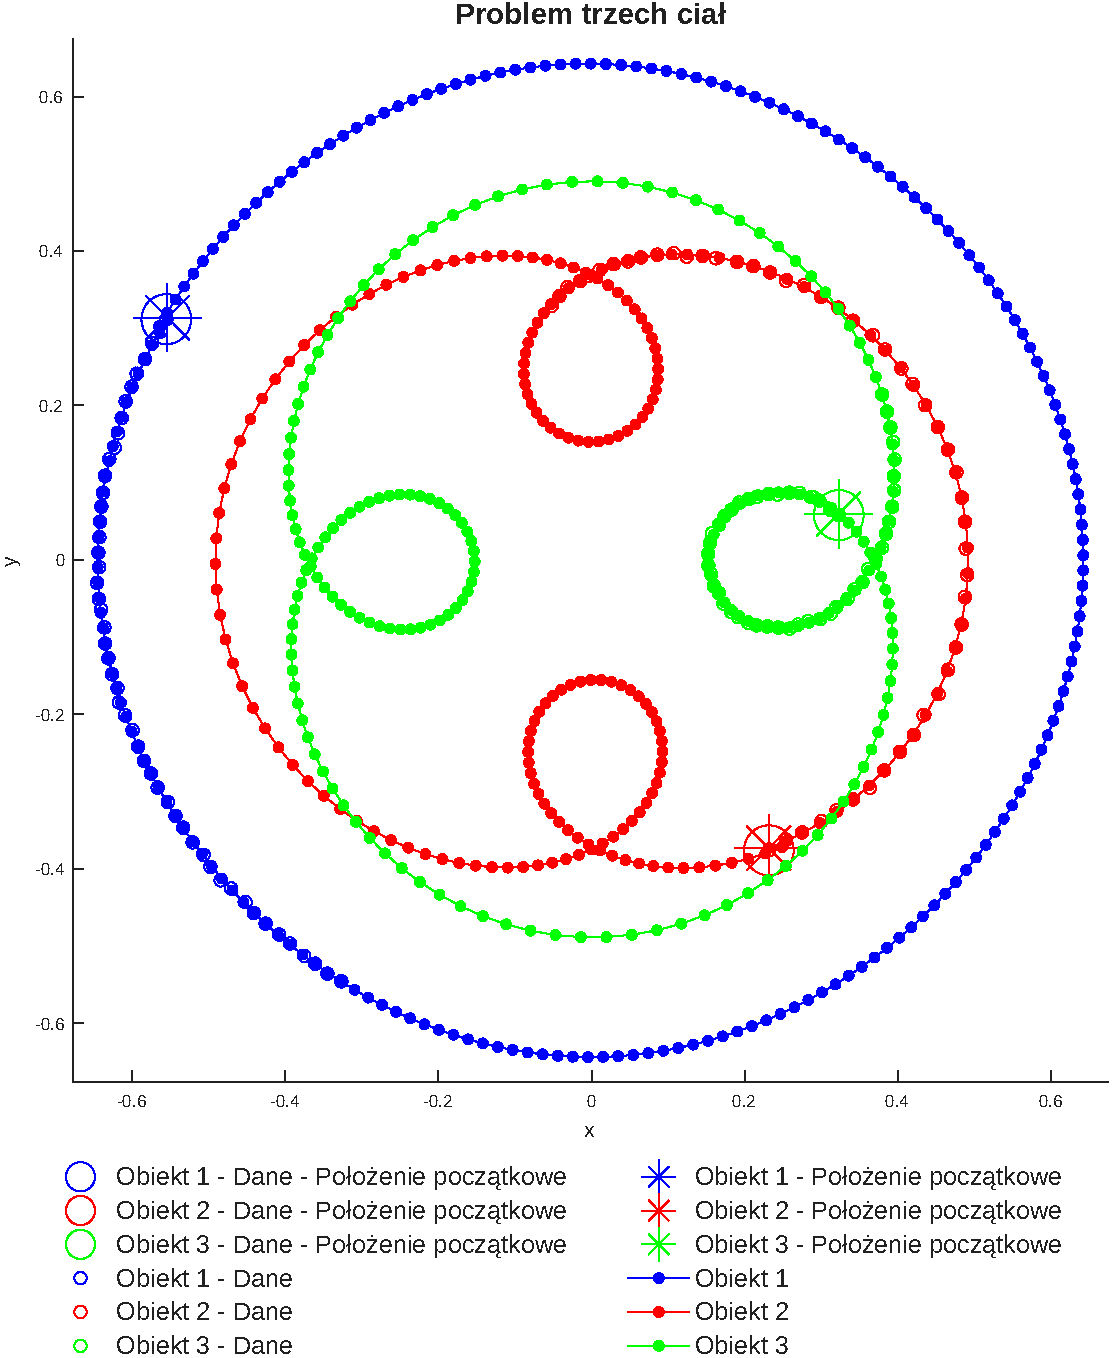
\includegraphics[scale=0.8]{orbity2.pdf}
	\caption{\normalsize Wyznaczone estymaty orbit obiektów}
	\label{fig:rys1} % Optional: Use this label for referencing
	\end{figure}

	\noindent
	Dla obliczonych estymatów położeń, zawartą w pliku \texttt{test\_solution\_30.p} funkcją\\ \texttt{test\_solution\_30}, obliczono wskaźnik dokładności rozwiązania $\Delta = 0.0169 < 0.02$.
	
	\newpage
	
	% Dyskusja wyników eksperymentów numerycznych
	\section{Dyskusja Wyników i Wnioski}

	Problem trzech ciał, będący jednym z klasycznych zagadnień mechaniki nieba oraz teorii chaosu, nie ma ogólnego rozwiązania analitycznego. Z tego względu, rozwiązania tego problemu są często badane numerycznie, z czego wynikają liczne problemy, na przykład dotyczące dokładności danych wejściowych. 
	W problemie trzech ciał, jakość danych pomiarowych ma kluczowe znaczenie dla dokładności uzyskiwanych wyników. Nawet niewielkie błędy w danych pomiarowych mogą prowadzić do znaczących odchyleń w trajektoriach obiektów. W związku z tym, proces optymalizacji parametrów początkowych miał kluczowe znaczenie dla uzyskania precyzyjnych wyników. \\
	
	\noindent
	Podczas dopasowywania parametrów początkowych, kluczowym było wyznaczenie wartości iloczynu $Gm$ wystarczająco bliskiej wartości faktycznej. Drobne zmiany w wartości $Gm$, na przykład zmiana wartości $Gm \approx 0.361$ na $Gm = 0.360$ lub $Gm = 0.362$ (różnica mniejsza niż $0.3\%$) sprawia, że rozwiązanie przestaje być zadowalające. Choć dane pomiarowe położeń zawierały błędy, funkcja \texttt{fminsearch}, używająca algorytmu korzystającego z metody numerycznej Neldera-Meada do wyznaczania ekstremum, pozwoliła na uzyskanie zadowalających warunków początkowych. \\
	
	\noindent
	Zastosowanie funkcji \texttt{ode45}, korzystającej z jawnej metody Rungego-Kutty 4-go rzędu z poprawką (metoda Dormanda-Prince'a) z adaptacyjnym krokiem, do rozwiązania układu równań różniczkowych okazało się stabilne i skuteczne, nawet w kontekście chaotycznego charakteru problemu trzech ciał. Dzięki temu możliwe było uzyskanie zadowalająco dokładnych trajektorii obiektów w przyszłych momentach czasowych, wykraczających poza zakres danych pomiarowych. \\
	
	\noindent
	Uzyskane rozwiązanie jest jednym z periodycznych rozwiązań problemu trzech ciał.
	W układzie trzech ciał, periodyczność oznacza, że po pewnym czasie obiekty wracają do swoich początkowych pozycji i prędkości, co prowadzi do cyklicznego powtarzania się trajektorii. Chociaż układ trzech ciał jest w ogólności chaotyczny i wrażliwy na początkowe warunki, istnieją szczególne przypadki, w których rozwiązanie jest periodyczne. Takie trajektorie są stabilne w sensie, że ich kształt i zachowanie powtarzają się w równych odstępach czasu.

	
	\newpage
	
	% Lista źródeł informacji
	\section*{Bibliografia}
	\addcontentsline{toc}{section}{Bibliografia}
	\begin{enumerate}
		\item Dokumentacja MATLAB: \url{https://www.mathworks.com/help/matlab}.
		\item \url{https://en.wikipedia.org/wiki/Three-body\_problem}
	\end{enumerate}
	
	\newpage
	
	% Listing opracowanych programów
	\section*{Listing Programów}
	\addcontentsline{toc}{section}{Listing Programów}
	
	\subsection*{plik: \texttt{Projekt2.m}}\vspace{-0.5em}
	\lstinputlisting{../Projekt2.m}
	\subsection*{plik: \texttt{ApproximateDerivative.m}}\vspace{-0.5em}
	\lstinputlisting{../ApproximateDerivative.m}
	\subsection*{plik: \texttt{ODEFunction.m}}\vspace{-0.5em}
	\lstinputlisting{../ODEFunction.m}
	\subsection*{plik: \texttt{Criterium.m}}\vspace{-0.5em}
	\lstinputlisting{../Criterium.m}
	\subsection*{plik: \texttt{ApproximateMass.m}}\vspace{-0.5em}
	\lstinputlisting{../ApproximateMass.m}
	\subsection*{plik: \texttt{Visualize.m}}\vspace{-0.5em}
	\lstinputlisting{../Visualize.m}

\end{document}
